\begin{figure}[t]
\centering
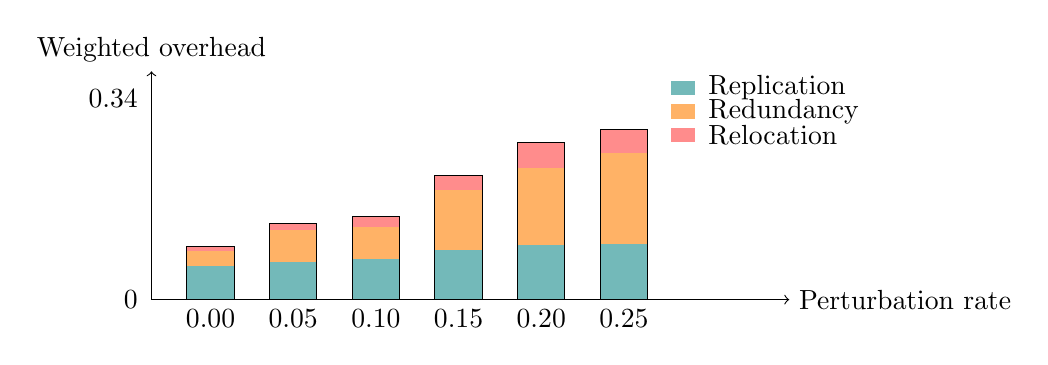
\begin{tikzpicture}[x=1cm,y=1cm]
\draw[->] (0.55,0.45) -- (8.65,0.45) node[right] {Perturbation rate};
\draw[->] (0.55,0.45) -- (0.55,3.35) node[above] {Weighted overhead};
\node[left] at (0.50,0.45) {0};
\node[left] at (0.50,3.00) {0.34};
\fill[teal!55] (1.00,0.45) rectangle (1.60,0.88);
\fill[orange!60] (1.00,0.88) rectangle (1.60,1.07);
\fill[red!45] (1.00,1.07) rectangle (1.60,1.12);
\draw (1.00,0.45) rectangle (1.60,1.12);
\node[below] at (1.30,0.45) {0.00};
\fill[teal!55] (2.05,0.45) rectangle (2.65,0.93);
\fill[orange!60] (2.05,0.93) rectangle (2.65,1.33);
\fill[red!45] (2.05,1.33) rectangle (2.65,1.42);
\draw (2.05,0.45) rectangle (2.65,1.42);
\node[below] at (2.35,0.45) {0.05};
\fill[teal!55] (3.10,0.45) rectangle (3.70,0.97);
\fill[orange!60] (3.10,0.97) rectangle (3.70,1.37);
\fill[red!45] (3.10,1.37) rectangle (3.70,1.50);
\draw (3.10,0.45) rectangle (3.70,1.50);
\node[below] at (3.40,0.45) {0.10};
\fill[teal!55] (4.15,0.45) rectangle (4.75,1.08);
\fill[orange!60] (4.15,1.08) rectangle (4.75,1.84);
\fill[red!45] (4.15,1.84) rectangle (4.75,2.03);
\draw (4.15,0.45) rectangle (4.75,2.03);
\node[below] at (4.45,0.45) {0.15};
\fill[teal!55] (5.20,0.45) rectangle (5.80,1.14);
\fill[orange!60] (5.20,1.14) rectangle (5.80,2.12);
\fill[red!45] (5.20,2.12) rectangle (5.80,2.45);
\draw (5.20,0.45) rectangle (5.80,2.45);
\node[below] at (5.50,0.45) {0.20};
\fill[teal!55] (6.25,0.45) rectangle (6.85,1.16);
\fill[orange!60] (6.25,1.16) rectangle (6.85,2.31);
\fill[red!45] (6.25,2.31) rectangle (6.85,2.61);
\draw (6.25,0.45) rectangle (6.85,2.61);
\node[below] at (6.55,0.45) {0.25};
\fill[teal!55] (7.15,3.05) rectangle (7.45,3.23);
\node[right] at (7.50,3.14) {Replication};
\fill[orange!60] (7.15,2.75) rectangle (7.45,2.93);
\node[right] at (7.50,2.84) {Redundancy};
\fill[red!45] (7.15,2.45) rectangle (7.45,2.63);
\node[right] at (7.50,2.54) {Relocation};
\end{tikzpicture}
\caption{Weighted non-access overhead for Online DQN across perturbation windows. Replication, redundancy, and relocation are intentionally small relative to access cost under the configured objective weights, but they grow with perturbation and make cache churn visible.}
\label{fig:generated_cost_components}
\end{figure}
